\documentclass[a4j,twocolumn]{ltjarticle}

%ページ設定
\setlength{\topmargin}{-10mm}
\setlength{\oddsidemargin}{-5mm}
\setlength{\evensidemargin}{-5mm}

\setlength{\textheight}{230mm}
\setlength{\textwidth}{170mm}
\setlength{\columnsep}{10mm}%コラムとコラムの間.よってコラムの横幅は(texwidth-columnsep)/2
\setlength{\footskip}{15mm}
%パッケージ
\usepackage{graphicx,color}
\usepackage{bm}
\usepackage{amsmath}
\usepackage{amsfonts}

%数学関数
\newcommand{\B}[1]{\bm #1} 
\newcommand{\s}[2]{{#1}\cdot{#2}} 
\newcommand{\R}{\mathbb{R}}
\newcommand{\M}{\mathbb{M}}
\newcommand{\df}[2]{\displaystyle{\frac{#1}{#2}}}
\newcommand{\qed}{
\begin{flushright}
\vspace{-8mm}
$\Box$
\end{flushright}
}

%ミニセクション
\newcommand{\minisection}[2]{\flushleft{\bf (#1)#2}\\ \ \ \ }

%図,表の名前変更
\renewcommand{\figurename}{Fig.}
\renewcommand{\tablename}{Tab.}

% refの拡張
\newcommand{\reffig}[1]{\figurename \ref{#1}}
\newcommand{\refeq}[1]{式(\ref{#1})}
\newcommand{\reftab}[1]{\tablename \ref{#1}}

% 図
\newcommand{\includefigure}[3]{
\begin{center}
\includegraphics[width=80mm]{#1}
\caption{#2}
\label{#3}
\end{center}
}
% 図 widthを変更したいときはこっち
\newcommand{\includefigurewidth}[4]{
\begin{center}
\includegraphics[width=#2]{#1}
\caption{#3}
\label{#4}
\end{center}
}

\usepackage{setspace} % setspaceパッケージのインクルード
\usepackage{enumitem}
\usepackage{graphicx}
\usepackage{amsmath}
%「Weekly Report」 
\newcommand{\Weekly}[5]{
\twocolumn[
 \begin{center}
  \bf
 第 #1 回 Weekly Report\\
 \huge
電気使用量予測のための深層学習手法\\

 \end{center}
 \begin{flushright}
  #2 月\ \ \  #3 日 \ \ \ #4 \\\
  #5
 \end{flushright}
]
}
%\setstretch{0.5} % ページ全体の行間を設定

\begin{document}

\Weekly{6}{5}{18}{(火)}{\ 小松 大起}
\section{はじめに}
\subsection{研究背景}
近年, 情報処理技術として知的処理技術の一つである深層学習が様々な分野で用いられている. 深層学習とは, ニューロンの層が多段に組み上げられたニューラルネットワークのことを指す.[1]ニューラルネットワークとは人間の脳の仕組みから着想を得たものであり, 神経回路網をコンピュータ上で表現しようと作られた数理的モデルである.深層学習で用いられる分野としては株価予想や人物認識や表情認識, 擬似的なデータを生成するアルゴリズムである GAN を用いた画像生成などに挙げられる画像処理, 話し言葉や書き言葉など我々が普段使うような自然言語を対象として, それらの言葉が持つ意味を解析する自然言語処理などがある.

\subsection{研究目的}

人間の認知は時間経過による視覚世界の変化の予測が可能である. 近年では実際に予測動画を作る研究も行われてきている.[2]電力使用量を予測することによる, 電気料金の予測が可能になると考えられる. 本研究では, 電力使用量を主データとし, 天気や気温が与えうる電力使用量の変化を考慮した電気使用料の予測を行うことを目的とする. 

\section{深層学習モデル}
\subsection{RNN}
\subsection{LSTM}

\section{活性化関数}
活性化関数とは, ニューロン間の移動に伴い入力値を別の数値に変換して出力するための関数のことである.
\subsection{ステップ関数}
ステップ関数は, 入力が 0 未満の場合には常に出力値が 0 となり, 0 以上の場合には常に出力値が 1 となるような関数を指す. ステップ関数は, パーセプトロンから用いられている関数であり入力 0 を起点として階段状のグラフを示す. この起点を閾値と呼ぶ. 入力を $x$ として $f(x)$ を出力とすると数式は以下の式で表される.
\begin{equation}
f(x)= \begin{cases}
0, & (x < 0)\\
1, & (x \geq 1)
\end{cases}
\end{equation}

\section{事前実験}
\subsection{用いるモデル構造}
本実験では, RNN 及び LSTM を用いて電力使用量の予測を行う. また, 予測に用いるデータは電力使用量のみを用いる. 本実験では, 予測結果は全て t+1 ステップ後の結果を表している. 
\subsection{用いるデータ}
本実験で用いるデータは, 東京電力パワーグリッド株式会社が提供している 2016 年 4 月から 2020 年 12 月までの電力使用量のデータであり, 年度, 日にち, 1 時間ごとの電力使用量(万 Kw)の3 要素が csv ファイルで提供されている. 2016 年は 4 月からのデータのため, 6600rows * 3columns, 2017 年から 2019 年は 8760rows * 3columns, 2020 年は閏年のために1日分多いため 24 列多い 8784rows * 3columns のデータである. また, 用いるデータの一例を図 0 に示す. これらのデータの日にちと時間を結合させて日時のデータとする. また, その際に日付と時間が並んでいるだけの文字列であるので, Python のデータ解析用ライブラリである pandas を用いて文字列を日付データに変換する. その例を図 0 に示す. また, データを可視化してグラフにしたものの例として 2020 年のグラフ及び, 2020 年 4 月 1 日(水曜日)と, 2020 年 4 月 5 日(日曜日)のグラフの比較を図 0 と図 0 にそれぞれ示す. 2020 年のグラフからわかることは夏と冬に電力使用量のピークを迎え, 春と秋に使用量は減っていることがわかる. 時間帯によっても使用料の増減があることが日のグラフを見ることでわかる. 深夜から朝にかけて段々と使用料が増えていき, 人々が活動を行なっているであろう 9 時ごろから 18 時ごろまで使用量がピークで, そこから使用量が段々と下がっていることがわかる. また, 1 日は平日であるため活動時間は常に使用量が多いが, 5 日は日曜日のため活動時間にばらつきがあると思われ,ピークは夜のみとなっていることがわかる. 

\begin{figure}[hb]
\centering
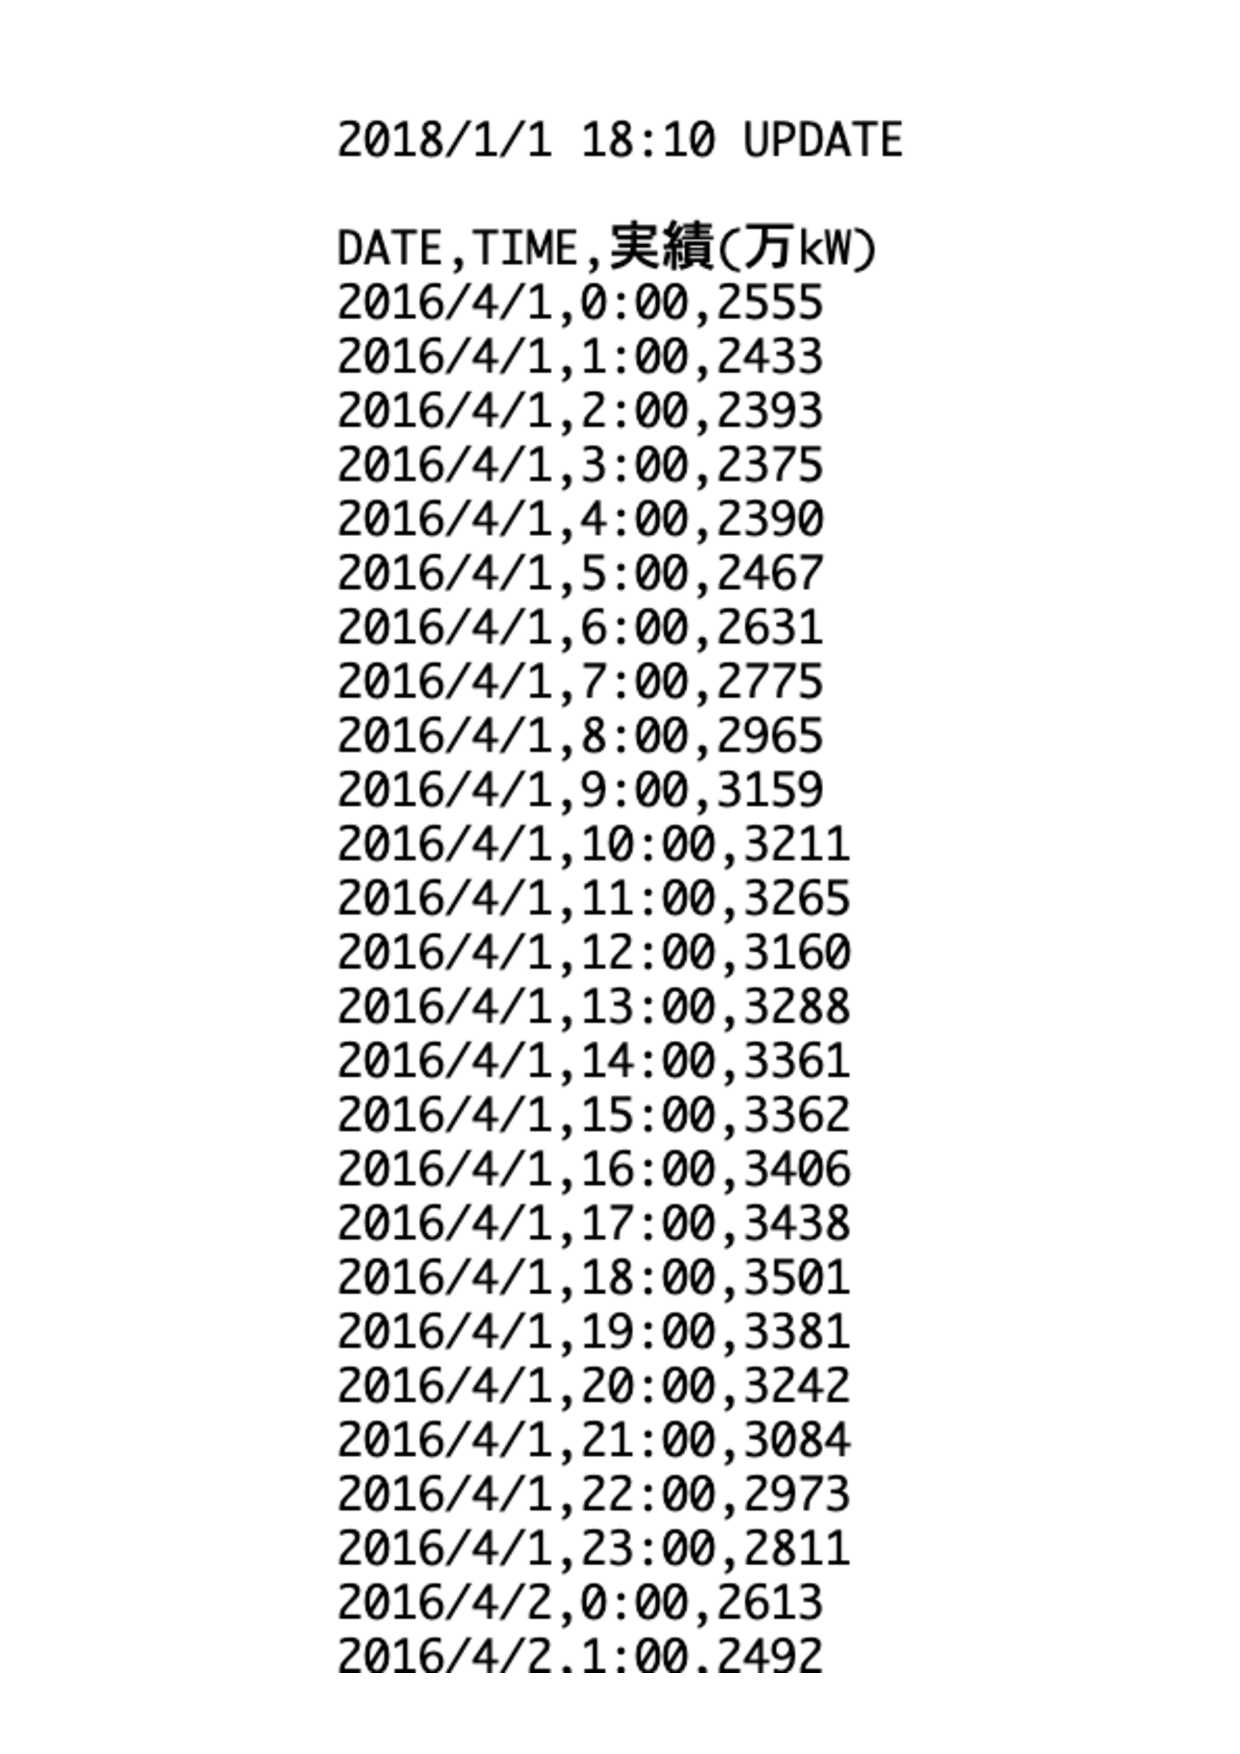
\includegraphics[scale=0.5]{exe_csv.pdf}
 \caption{用いる電力使用量データ例}
\end{figure}

\begin{figure}[hb]
\centering
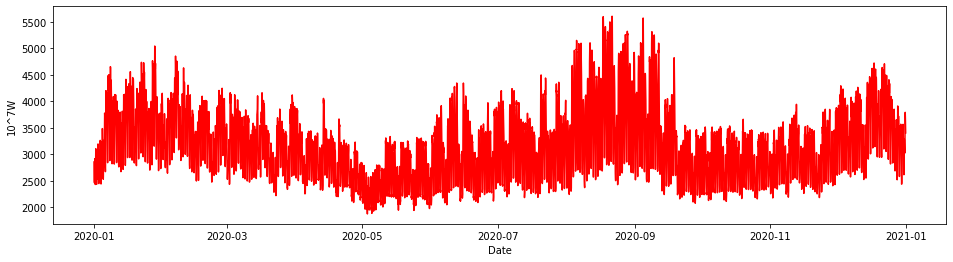
\includegraphics[scale=0.5]{2020_W.png}
 \caption{2020 年の電力使用量のグラフ}
\end{figure}

\begin{figure*}[hb]
\centering
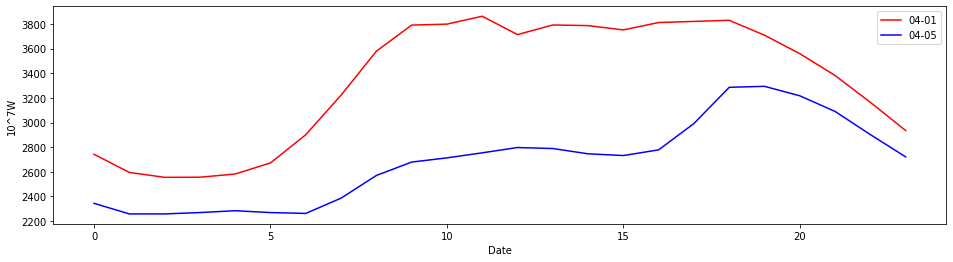
\includegraphics[scale=0.5]{compere_day.png}
 \caption{2020 年 4 月 1 日と 4 月 5 日の電力使用量の比較}
\end{figure*}

\subsubsection{RNN}
keras の simpleRNN というモデルを用いて訓練データと試験データを 8:2 に分けて学習データの作成を行った. 中間層 1 層, 隠れニューロン数は 100 とした. また、その時の予測の結果を図 0 に示す.

%% \begin{figure*}[ht]
%% \begin{center}
%% 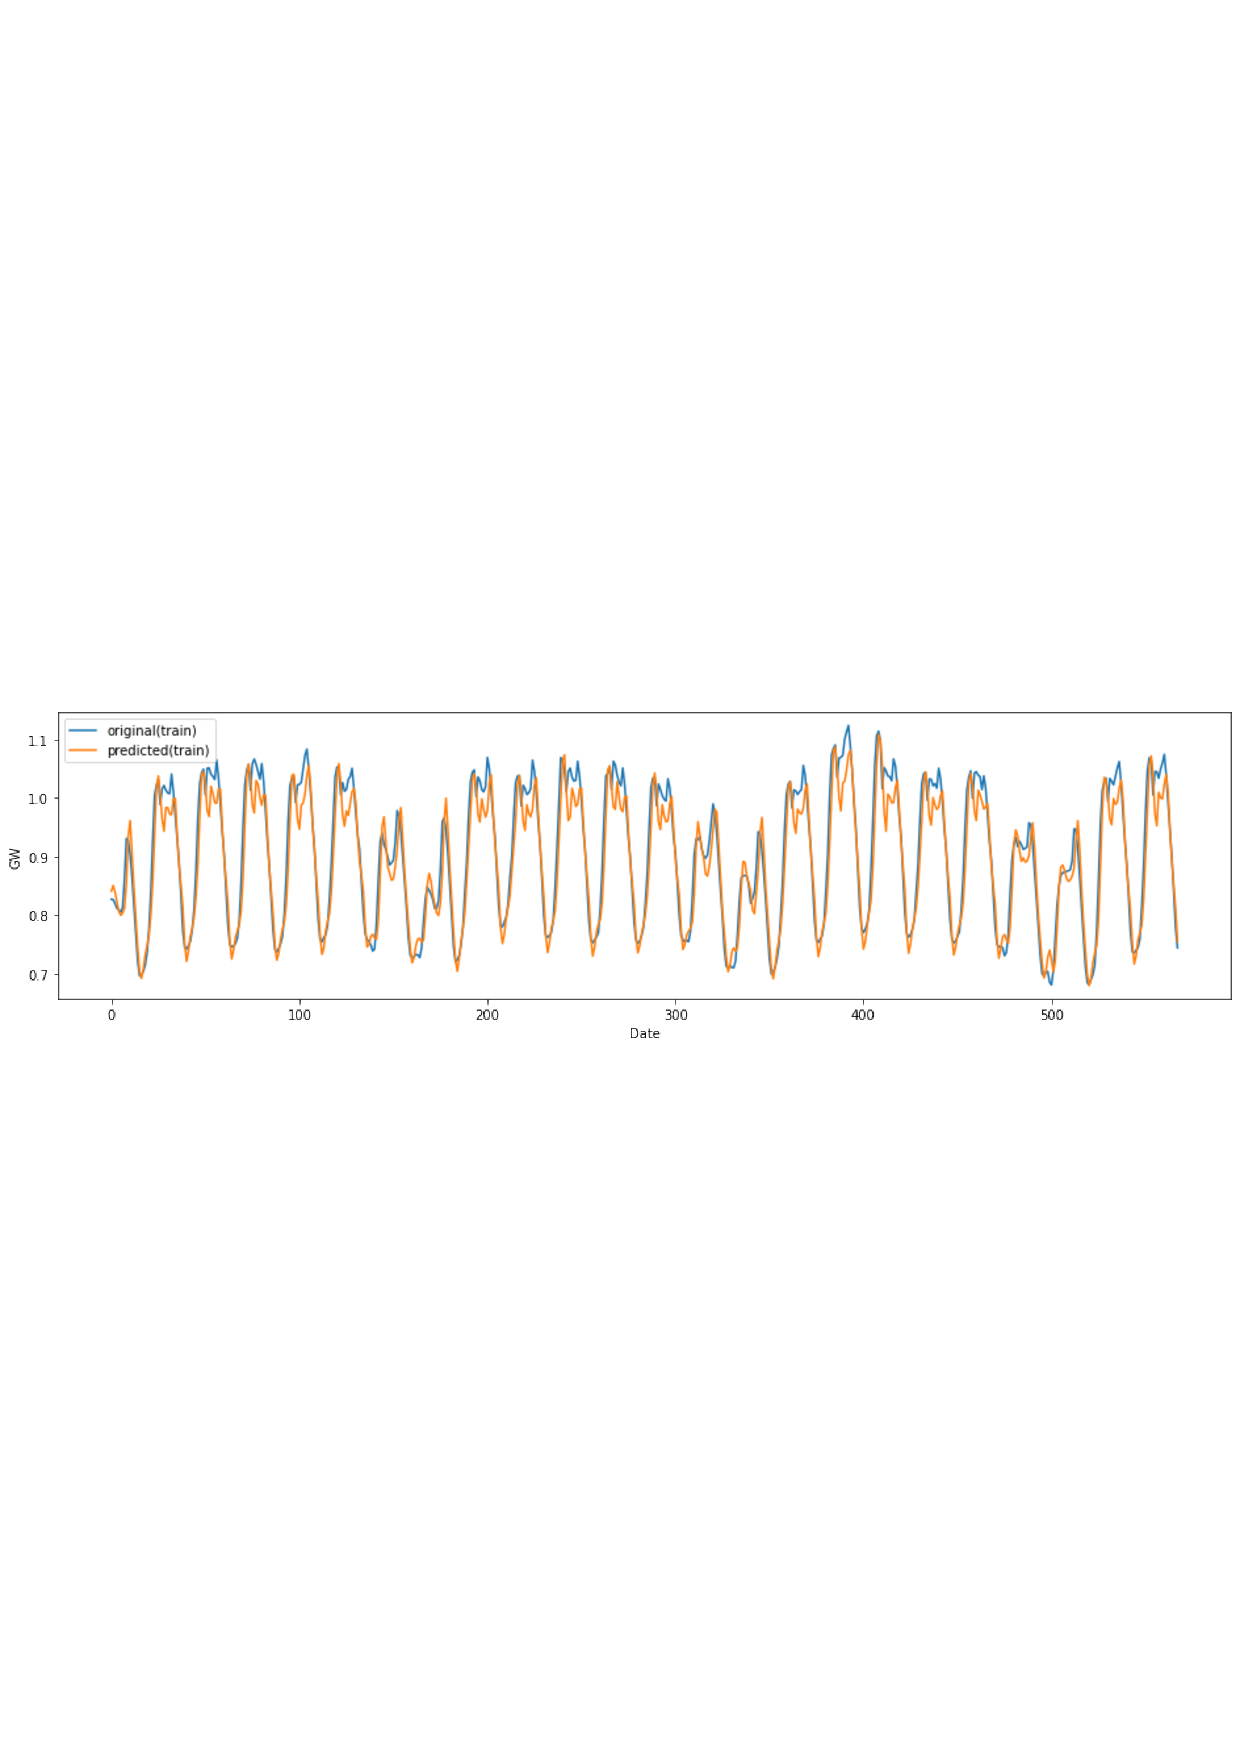
\includegraphics[scale=0.6]{rnn_pred_month.pdf}
%% \end{center}
%% \vspace{-80mm}
%% \caption{RNN 訓練データに対する予測結果}
%% \end{figure*}

%% \begin{figure*}[b]
%% \begin{center}
%% 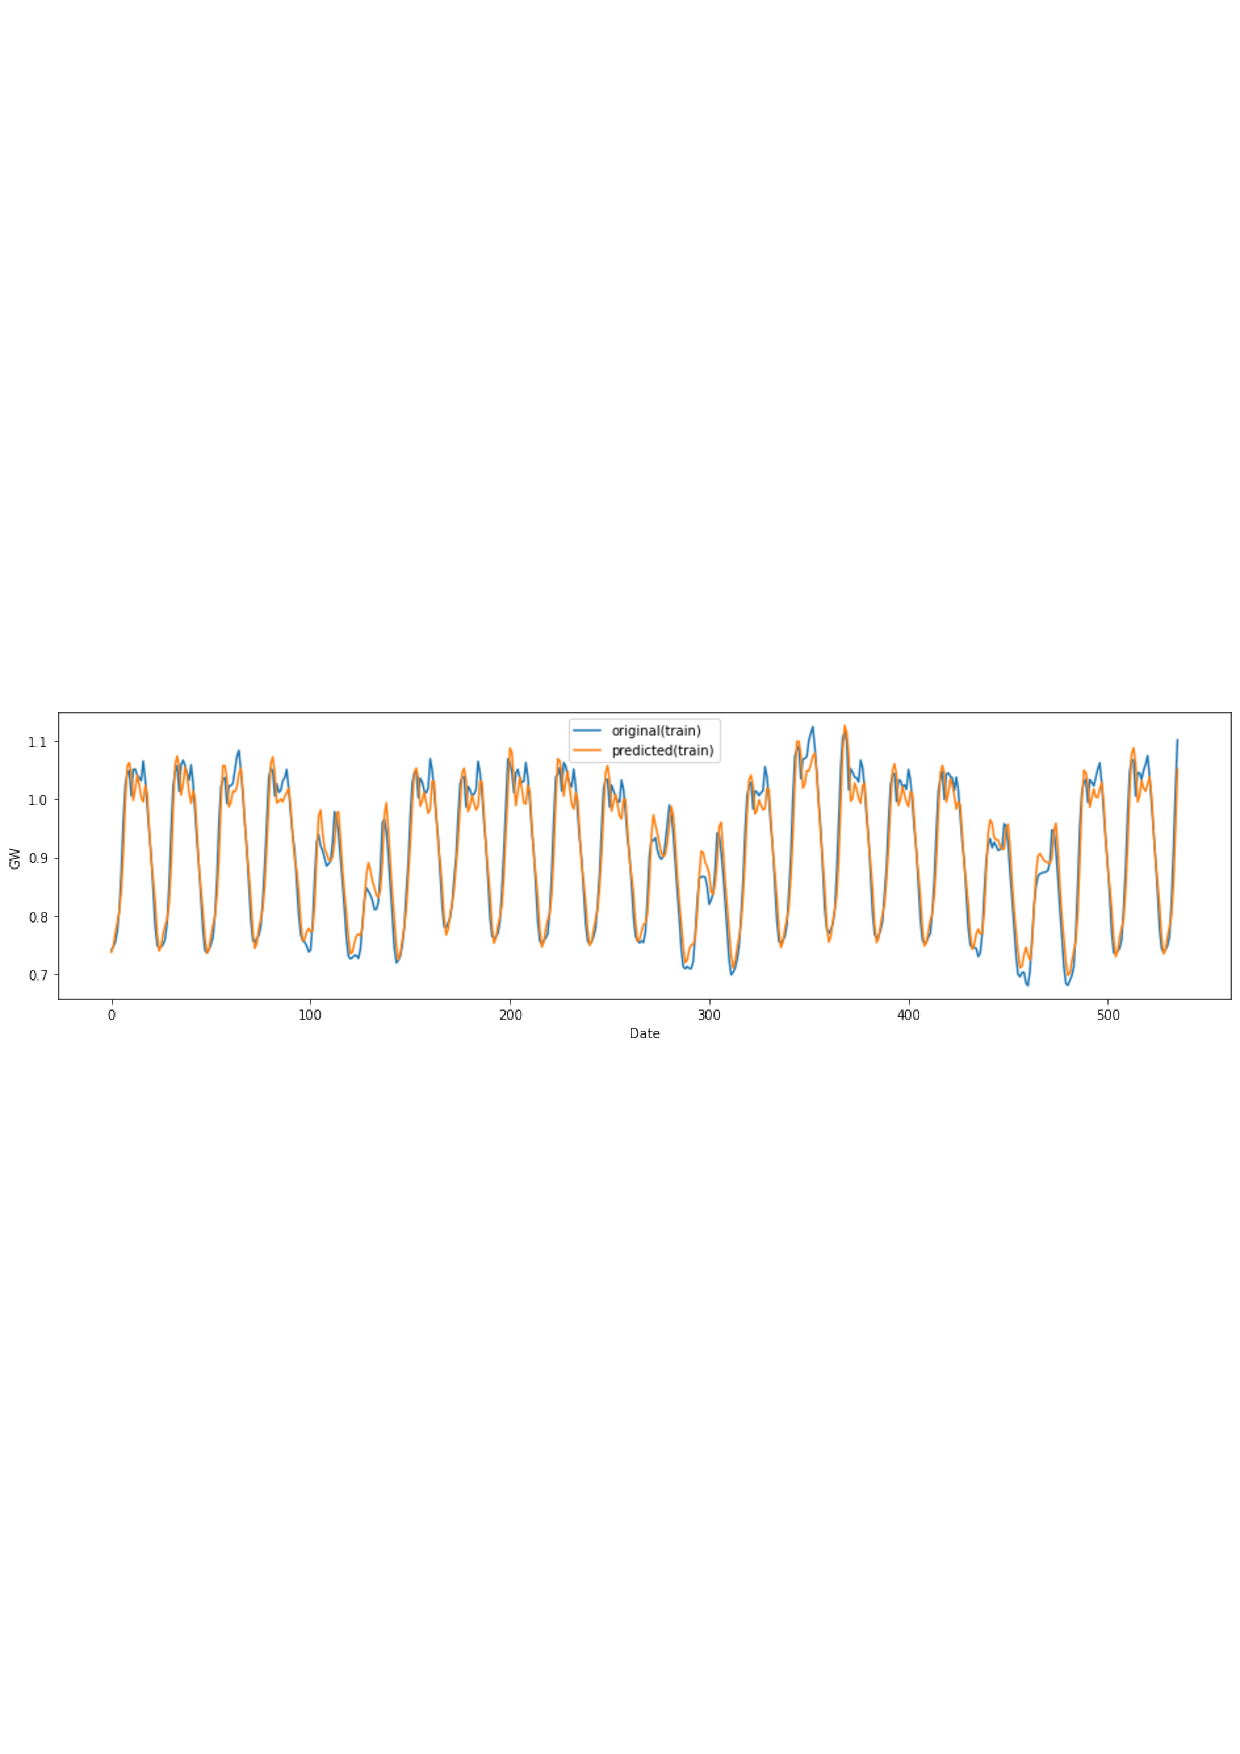
\includegraphics[scale=0.6]{lstm_pred_month.pdf}
%% \end{center}
%% \vspace{-80mm}
%% \caption{LSTM 訓練データに対する予測結果}
%% \end{figure*}

\subsubsection{LSTM}
RNN と同条件で予測を行った結果を以下の図に示す.

%% \begin{figure*}[ht]
%% \begin{center}
%% 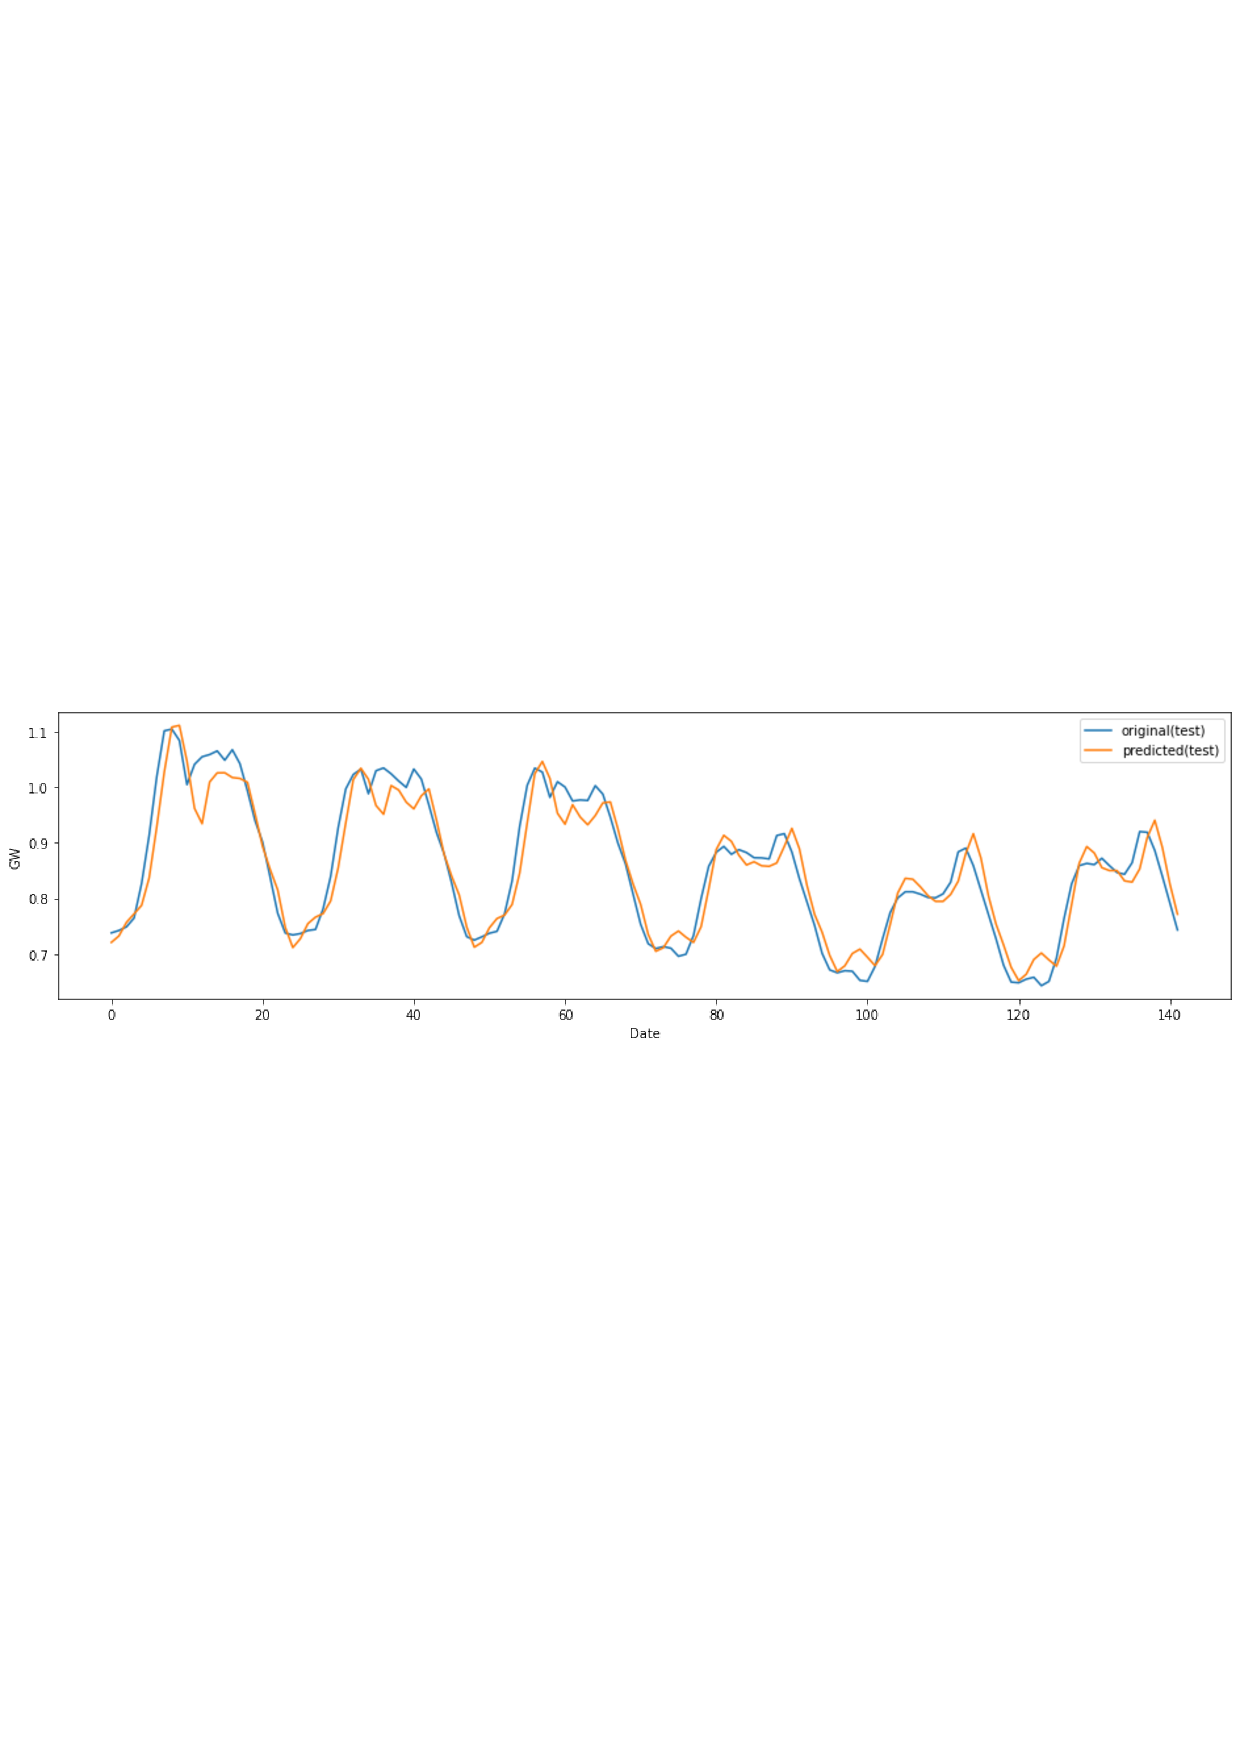
\includegraphics[scale=0.55]{rnn_pred_day.pdf}
%% \vspace{-75mm}
%% \caption{RNN テストデータに対する予測結果}
%% \end{center}
%% \end{figure*}

%% \begin{figure*}[phb]
%% \begin{center}
%% 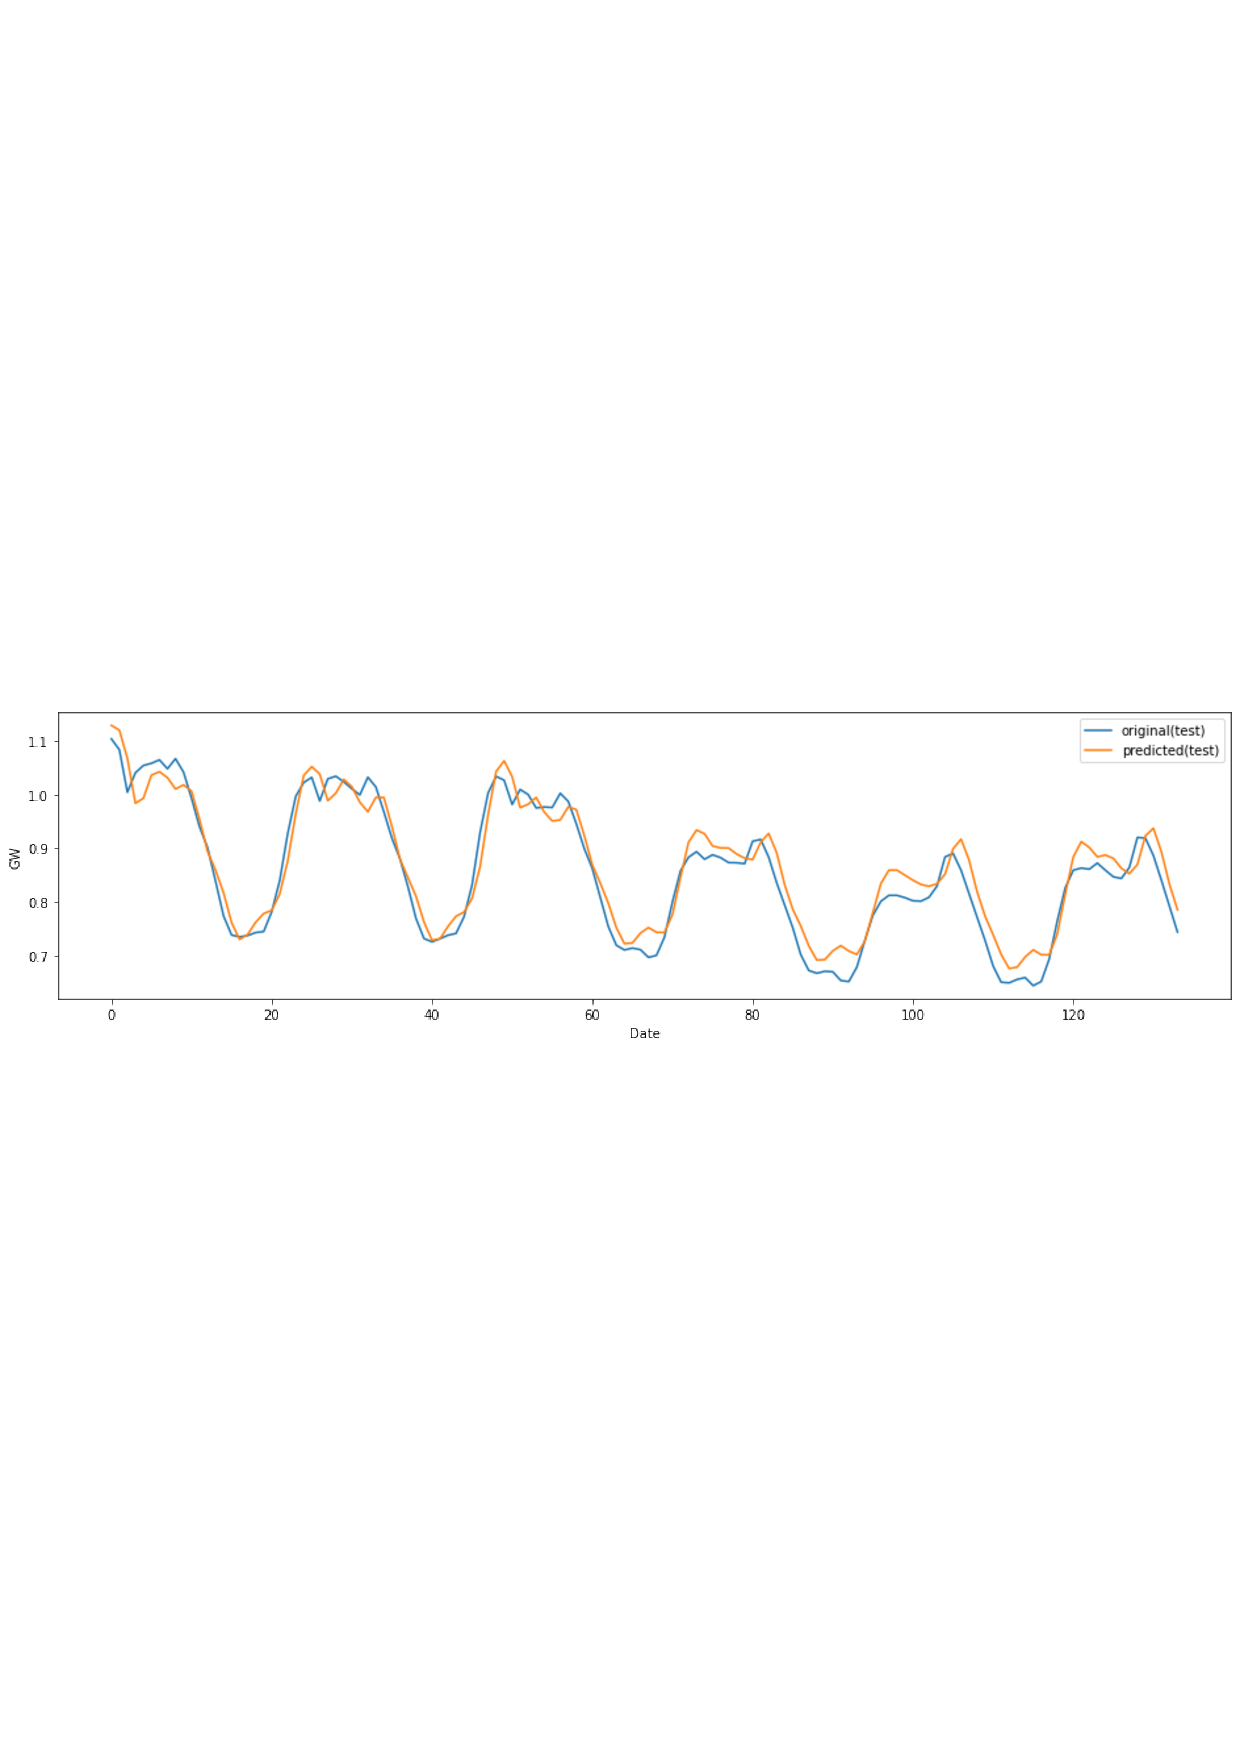
\includegraphics[scale=0.55]{lstm_pred_day.pdf}
%% \vspace{-75mm}
%% \caption{LSTM テストデータに対する予測結果}
%% \end{center}
%% \end{figure*}

\subsection{予測結果}

\section{用いる追加データ}
本研究では, 電力使用力の予測を天気, 気温などの外的要因から行うことを目的とする.
国土交通省の気象庁がホームページで公開している気温, 天気の情報を用いる.
また, そのデータの例を図 0 に示す. 天気予報による天気の予測と実際の電気使用量の関連性を調べる. 天気概況をグラフに示す.品質番号は 8 を最大として利用上注意が必要がどうかを示す値である. 均質番号は番号により観測環境の違いを表している. この値が違う場合には, 同列のデータとして扱うことは難しい. 

\begin{figure*}[phb]
\centering
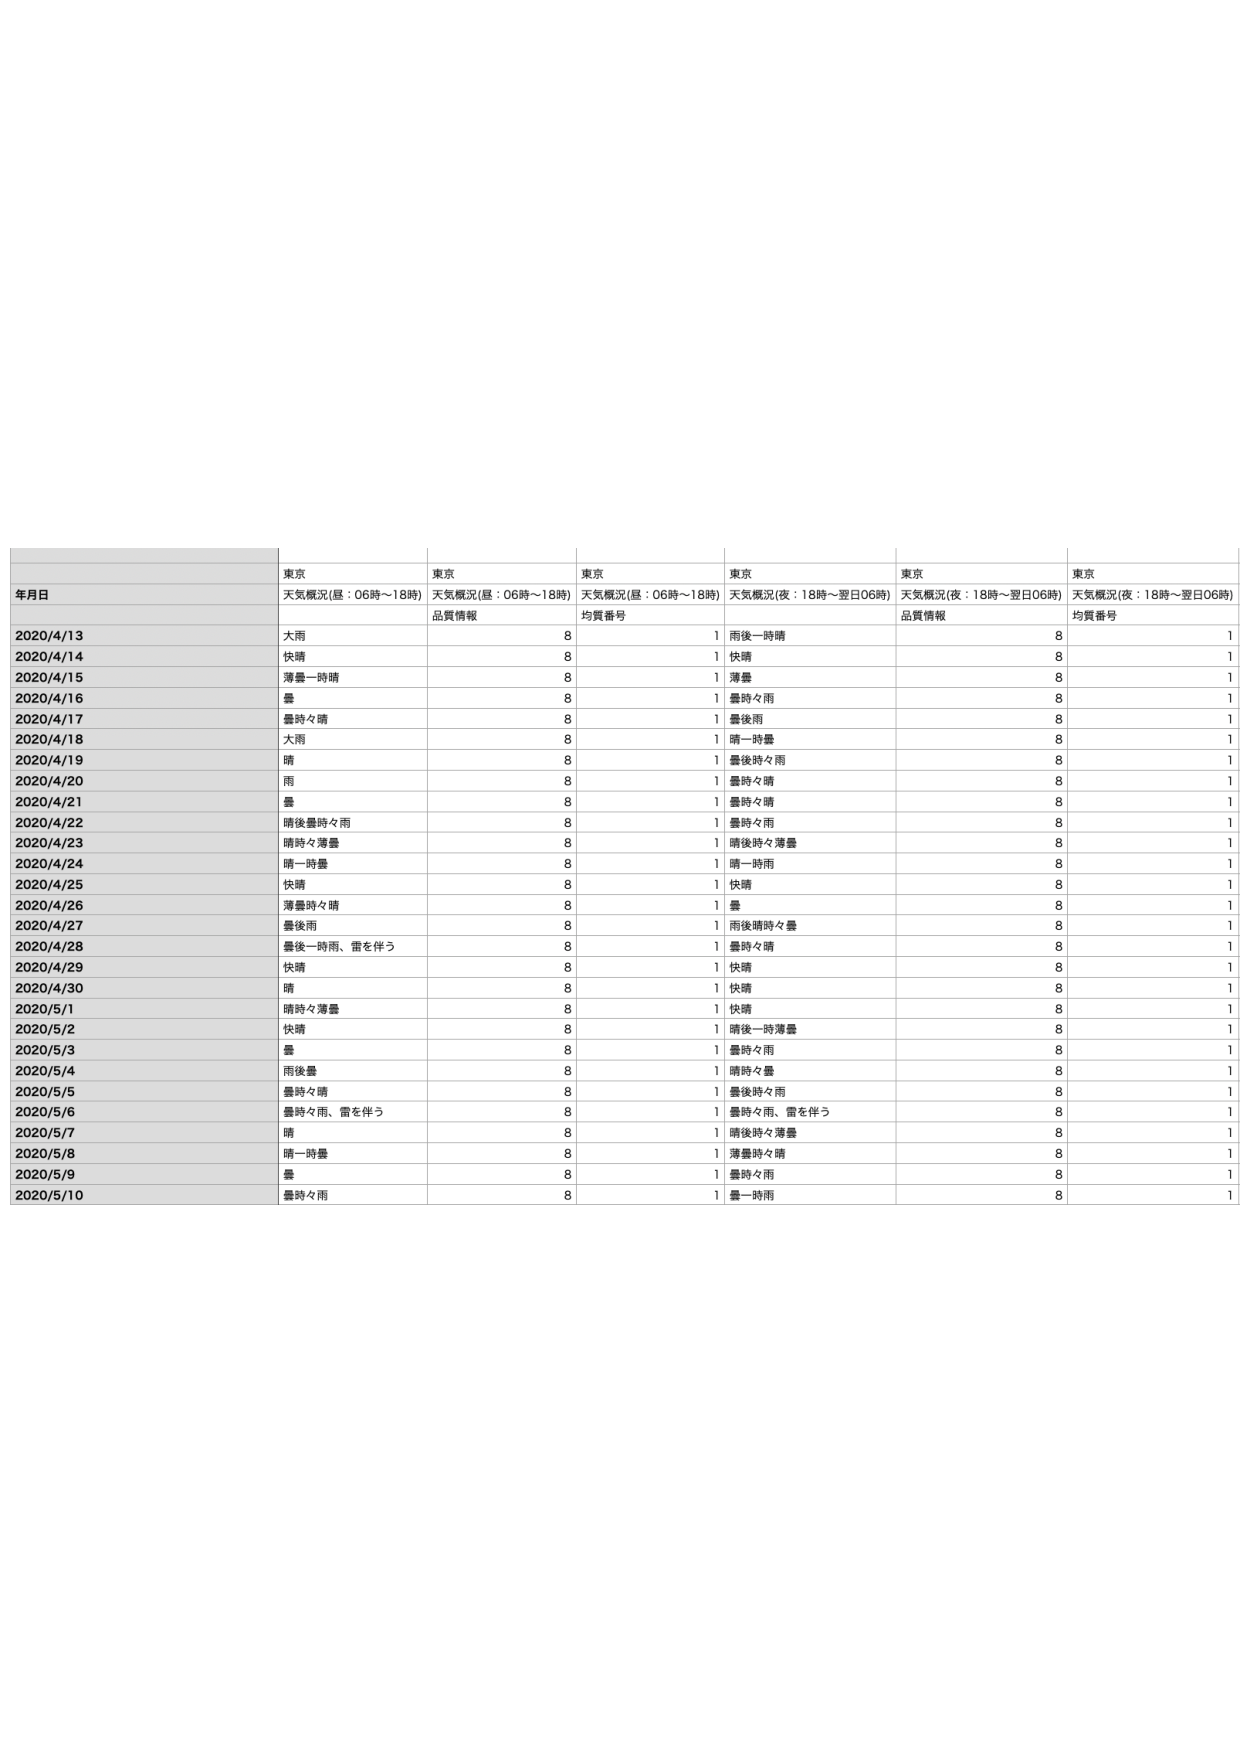
\includegraphics[scale=0.8]{exe_wether.pdf}
\caption{東京都における天気データ例}
\end{figure*}

\begin{figure}[hb]
\centering
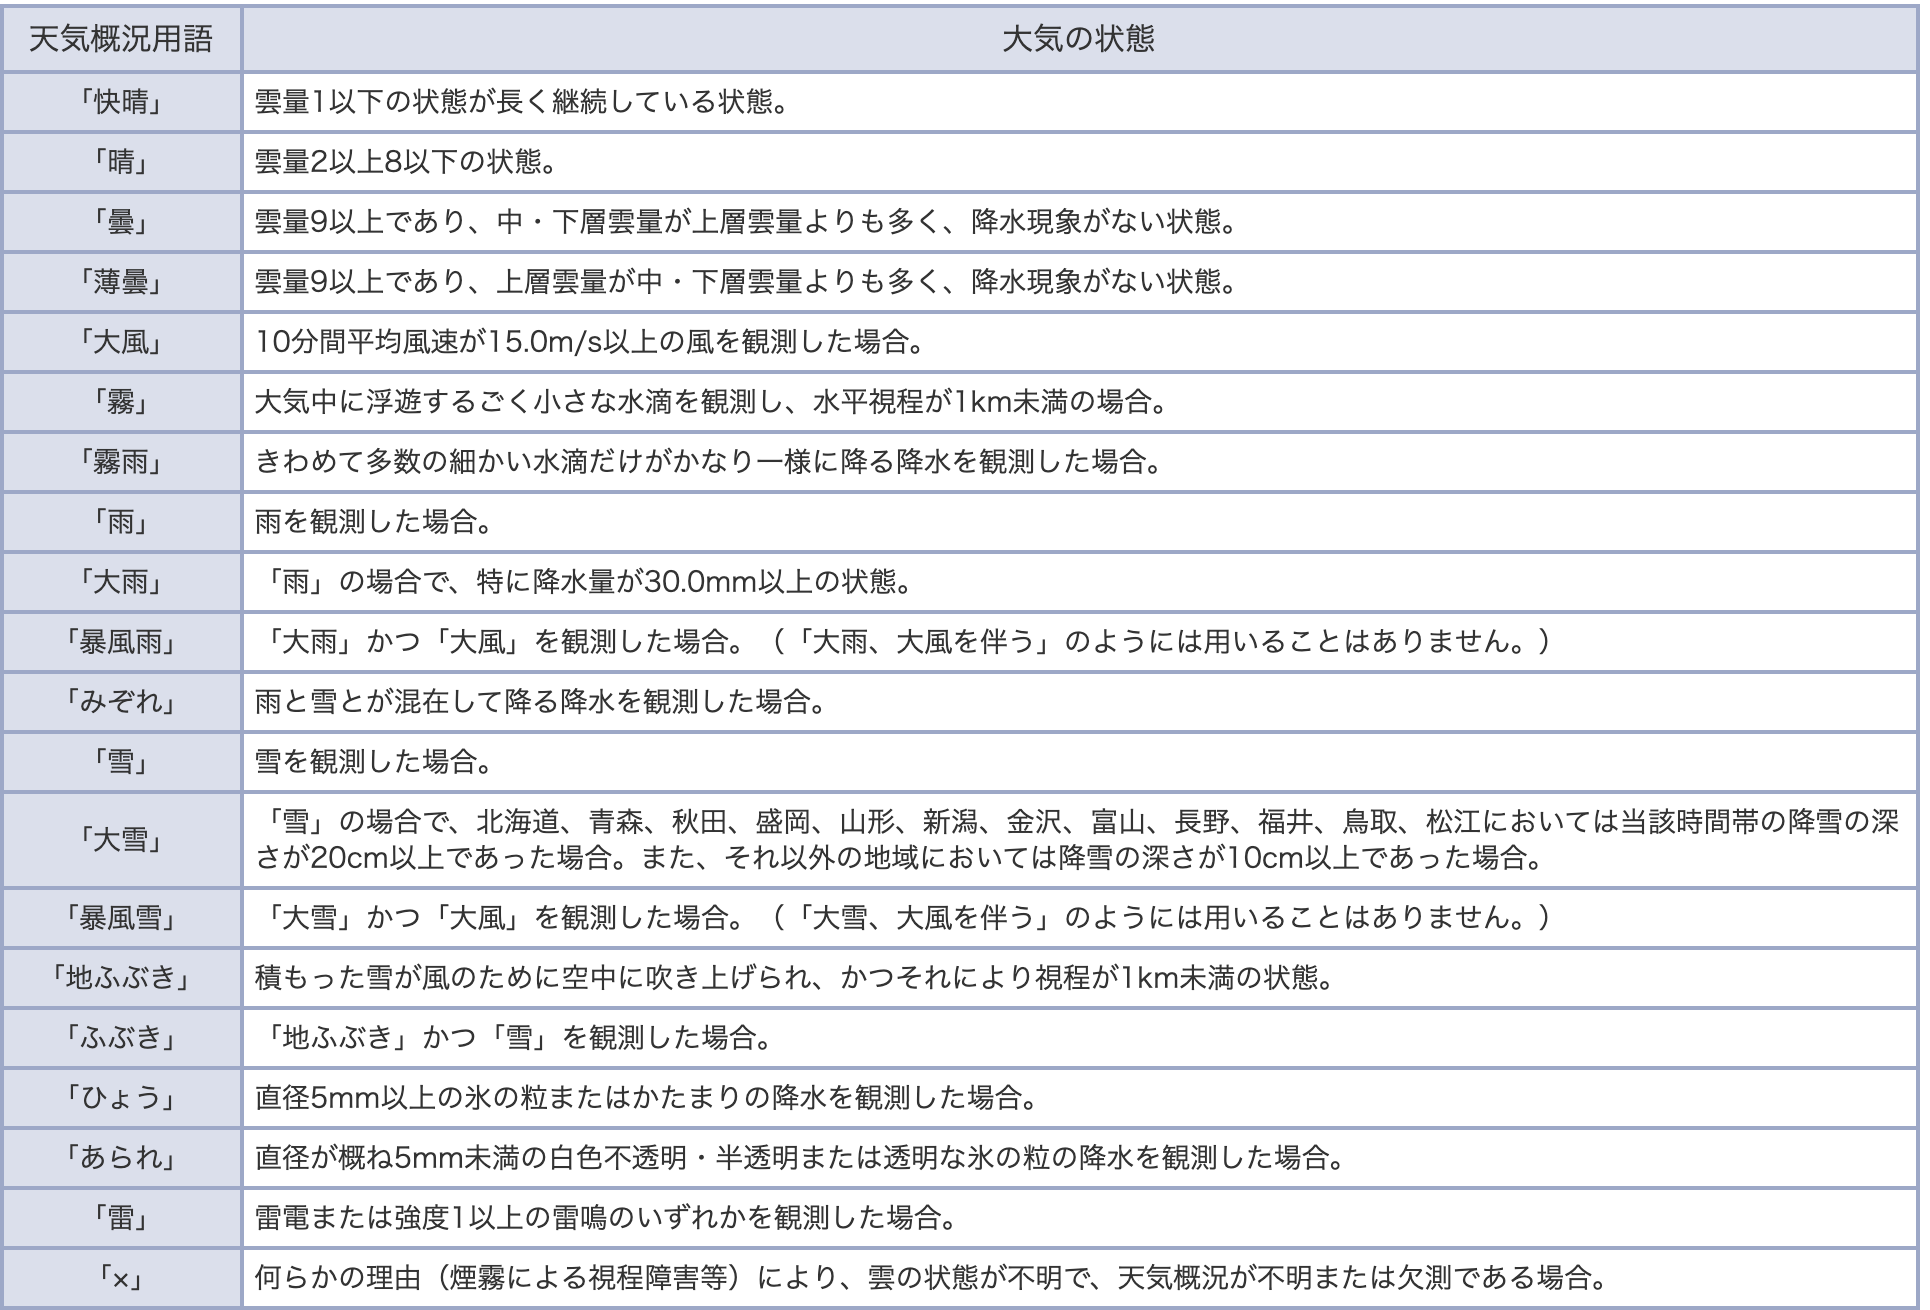
\includegraphics[scale=0.5]{wether.png}
 \caption{天気概況用語一覧}
\end{figure}

%\section{先週までの作業}
%\begin{itemize}
%
%\end{itemize}

\section{今週の作業}
\begin{itemize}
        \item 天気概況用語をみながら, 天気に評価値をつける. 天気を数値化してみているサイトや, 論文などを参考にしてみる. 
        \item 急激に数値が変わる点を確実に予測したいが, そうするにはどうしたら良いかを考える. 
\end{itemize}

\section{来週以降の作業}
\begin{itemize}
         \item 
\end{itemize}

\section{参考文献}
[1]浅川伸一. python で体験する深層学習. コロナ社, 2016.
[2]William Lotter, Gabriel Kreiman, David Cox, “Deep Predictive Coding Networks for Video Prediction and Unsupervised Learning”, ICLR, 2017



\end{document}
